  \documentclass[xcolor=svgnames,dvipsnames,table, hyperref=pdftex, mathserif, presentation]{beamer}
\usepackage{amsmath,amssymb,amsfonts,amsthm}
\usepackage{ctex}
\setCJKsansfont{KaiTi}% 文泉驿的黑体
\usepackage{graphics}
\usepackage{graphicx}
\usepackage{xcolor}
\usepackage{wasysym}
\usepackage{bbm}
\usepackage{url}
\usepackage{beamerleanprogress}
\usepackage{tikz-dependency}
\usepackage{tikz-qtree}
\usepackage{hhline}
\usepackage{fancyvrb}
\usepackage{mathrsfs}
\usepackage{alltt}
% for uml charts
\usepackage{tikz}
\usetikzlibrary{calc,arrows.meta, graphs, trees, shapes, positioning, automata,
shapes.geometric, shapes.multipart, er, patterns, decorations.markings, intersections, decorations.text}
\usepackage{tikz-uml}

\usetheme{CambridgeUS}
%\usetheme{Pittsburgh}
\usecolortheme{orchid} % seahorse  orchid rose
\setbeamertemplate{blocks}[rounded][shadow=true]
\AtBeginSection[]{%
  \begin{frame}<beamer>
    \frametitle{Outline}
      \tableofcontents[current] 
    \end{frame}
  \addtocounter{framenumber}{-1}% If you don't want them to affect the slide number
}
\AtBeginSubsection[]
{
  \begin{frame}
  \frametitle{Outline}
    \tableofcontents[currentsection,currentsubsection]
  %\tableofcontents[sectionstyle=show/hide,subsectionstyle=hide/show/hide]
  \end{frame}
  \addtocounter{framenumber}{-1}% If you don't want them to affect the slide number
}
\newcommand{\setof}[1]{\ensuremath{\left \{ #1 \right \}}}
\newcommand{\tuple}[1]{\ensuremath{\left \langle #1 \right \rangle }}
\newcommand{\red}[1]{\textcolor{red}{#1}}
\newcommand{\brown}[1]{\textcolor{brown}{#1}}
\newcommand{\green}[1]{\textcolor{green}{#1}}
\newcommand{\blue}[1]{\textcolor{blue}{#1}}
\newcommand{\cyan}[1]{\textcolor{cyan}{#1}}


\setbeamerfont{note page}{size=\footnotesize}

%gets rid of navigation symbols
%\setbeamertemplate{navigation symbols}{}

\begin{document}

\title[GloVe]{GloVe: Global Vectors for Word Representation \[EMNLP 2014)\]}

\institute[icst@pku]{
  Stanford
}
\author[Han Zhe]{
  Jeffrey Pennington \\
  Richard Socher \\
  Christopher D. Manning \\
}

\frame[t,plain]{ \titlepage } % [t,plain]

\frame{
  \frametitle{ Glo(bal)Ve(ctor)  }
  
   \begin{itemize}
      \item 词向量模型
	  \begin{itemize}
	   \item global matrix factorization (LSA)
	   \item local context window (skip-gram)
	  \end{itemize}

      \item word2vec的实现方式

      \item GloVe
	  \begin{itemize}
	   \item 模型(目标函数)
	   \item 对比skip-gram
	   \item 复杂度分析
	  \end{itemize}
      
      \item 实验
	  \begin{itemize}
	   \item Word analogies (A-B=C-?)
	   \item Word Similarity
	   \item Named entity recognition
	  \end{itemize}
	  
   \end{itemize}

}


\frame{
  \frametitle{词向量模型}
  global matrix factorization
  \begin{itemize}
   \item 可以利用预料中出现频率信息,但是处理 A-B=C-? 问题效果不好
  \end{itemize}
  
  local context window
  \begin{itemize}
   \item 处理 A-B=C-? 效果很好,但是利用局部单词的左右窗口内词作为上下文信息,不能利用全局层面的共现信息
  \end{itemize}

  GloVe
  \begin{itemize}
   \item 综合
   \item 建立满足A-B=C-D的模型,利用共现信息(共现频率)作为权值标准,最优化模型误差
  \end{itemize}

}


\frame{
  \frametitle{vector models}
  \begin{block}{
  global matrix factorization}
  \begin{itemize}
   \item 可以利用预料中出现频率信息,但是处理 A-B=C-? 问题效果不好
  \end{itemize}
  \end{block}
  
  \begin{block}{
  local context window}
  \begin{itemize}
   \item 处理 A-B=C-? 效果很好,但是利用局部单词的左右窗口内词作为上下文信息,不能利用全局层面的共现信息
  \end{itemize}
  \end{block}

  \begin{block}{
  GloVe}
  \begin{itemize}
   \item (综合)建立满足A-B=C-D的模型,利用共现信息(共现频率)作为权值标准,最优化模型误差
  \end{itemize}
  \end{block}

}


\frame{
  \begin{columns}[c]
   \column{.15\hsize}
   \column{.7\hsize}
   \begin{block}{}
    \centering \Large word2vec的实现方式
   \end{block}

   \column{.15\hsize}
  \end{columns}

}

\frame{
  \frametitle{word2vec实现:CBOW}
  \begin{columns}[c]
   \column{0.4\hsize}
      \centering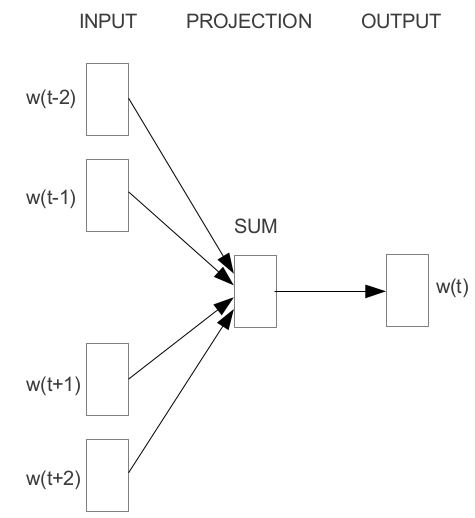
\includegraphics[width=0.55\hsize]{file/word2vec_CBOW.png} \\ 
      \vspace{1mm}
      \centering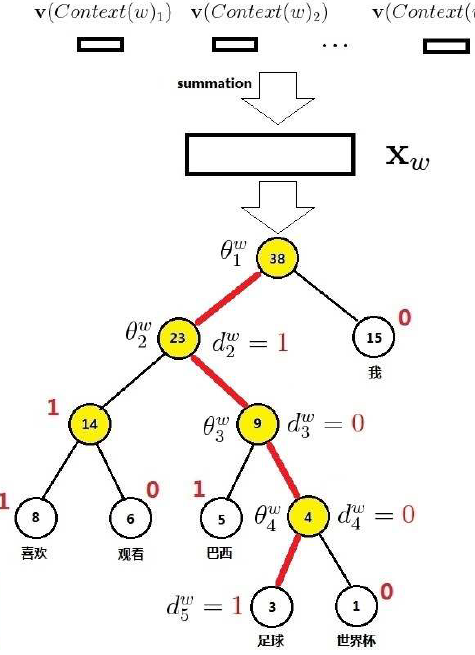
\includegraphics[width=0.75\hsize]{file/CBOW3.png}
      
   \column{0.58\hsize}
  \begin{block}{}
   \footnotesize
   \begin{itemize}
    \item 前后窗口(宽度1-4随机)内所有单词的词向量平均作为隐层词向量
    \item 所有单词按照词频构建huffman树,每个中间结点对应一个判别向量,和隐层词向量、目标词向量维数相同
    \item 每个中间结点的词向量和隐层词向量的点积做sigmod变换后的值,作为选择左分支(0)的概率,否则为走右支(1)的概率
    \item 每个单词是对应一个huffman编码\\
    \only<1>{
    \emph{足球fb(1001),观看(110)}
    $$p(fb|context(fb))=\prod_{j=2..5}p(d_j^w|X_w,\theta_{j-1}^w)$$
  \tiny
  \begin{equation}
    p(d_j^w|X_w,\theta_{j-1}^w)=
   \begin{cases}
   \sigma(x_w^T\theta_{j-1}^w) &\mbox{$d_j^w=0$}\\
   1-\sigma(x_w^T\theta_{j-1}^w) &\mbox{$d_j^w=1$}\\
   \end{cases}
  \end{equation}
  }
    \only<2>{
    \item 最优化 $\sum_{w\in C}\log p(c|context(c))$
    }
  
   \end{itemize}
  \end{block}
   
  \end{columns}
  
}

\frame{
  \frametitle{word2vec实现:Skip-gram}
  \begin{columns}[c]
   \column{0.4\hsize}
      \centering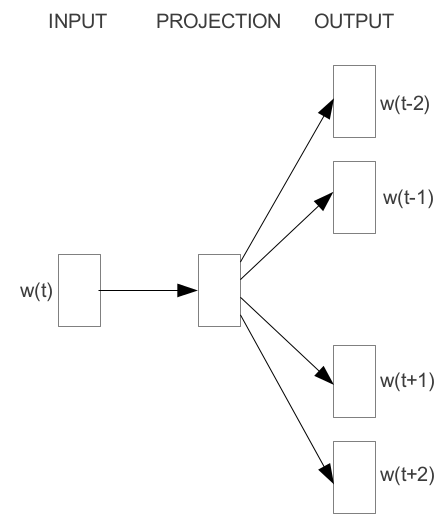
\includegraphics[width=0.55\hsize]{file/word2vec_sg.png} \\ 
      \vspace{1mm}
      \centering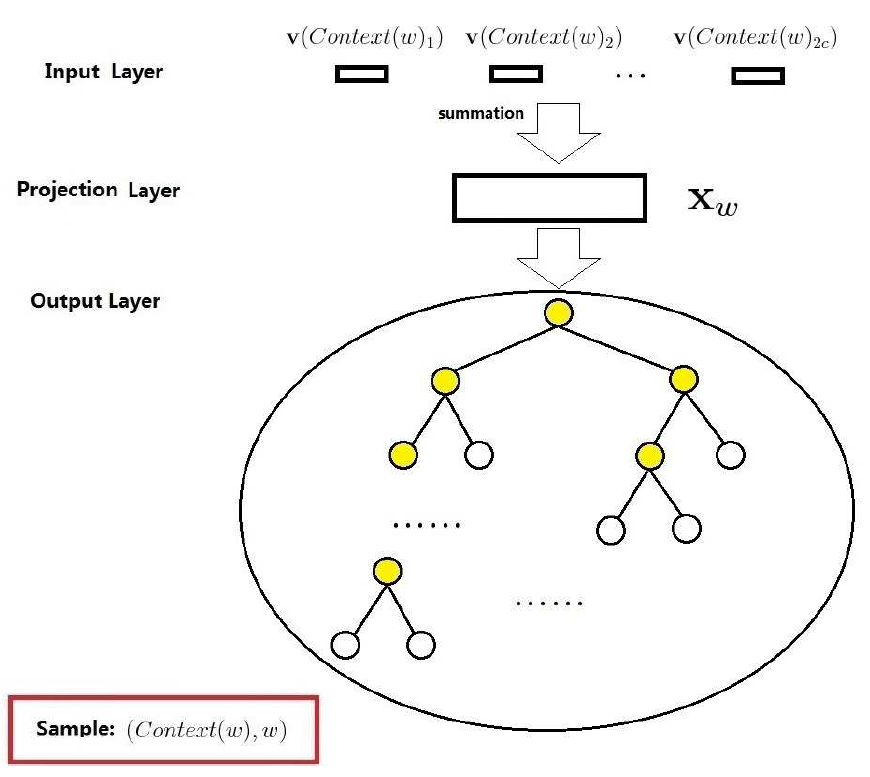
\includegraphics[width=0.75\hsize]{file/sg.png}
      
   \column{0.58\hsize}
  \begin{block}{}
   \footnotesize
   \begin{itemize}
    \item 类似CBOW
    \item 隐层就是输入的当前单词向量
    \item 不同的是每个隐层向量需要生成多个单词(窗口内的所有单词都预测,不分顺序)
	\begin{itemize}
	 \item 多一个$\prod$循环
	\end{itemize}
    \item 最优化 $\sum_{w\in C}\prod_{w_j \in window_c}\log p(w_j|c)$
  
   \end{itemize}
  \end{block}
   
  \end{columns}
}


\frame{
  \begin{columns}[c]
   \column{.15\hsize}
   \column{.7\hsize}
   \begin{block}{}
    \centering \Large GloVe Model
   \end{block}

   \column{.15\hsize}
  \end{columns}

}

\frame{
  \frametitle{GloVe Model}
  \begin{columns}[c]
   \column{0.4\hsize}
   \begin{block}{}
   \begin{itemize}
    \item $X_{ij}:word_j$作为$word_i$上下文出现次数
    \item $X_i=\sum_kX_{ik}$
    \item $P_{ij}=P(j|i)=X_{ij}/X_i$
    \item $F(w_i,w_j,\widetilde{w}_k)=P_{ik}/P_{jk}$
   \end{itemize}
   \end{block}
   
   \column{0.58\hsize}
   \begin{enumerate}
    \item 改用向量差别 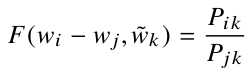
\includegraphics[width=0.4\hsize]{file/eq1.png}
    \item 保持线性结构 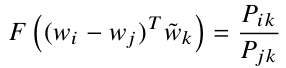
\includegraphics[width=0.45\hsize]{file/eq2.png}
    \item 我们采用$F=exp$或者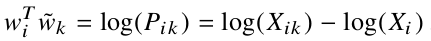
\includegraphics[width=0.5\hsize]{file/eq7.png},使得下面的式子成立\\
     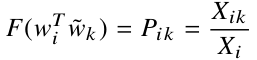
\includegraphics[width=0.35\hsize]{file/eq6.png} 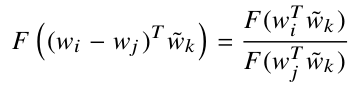
\includegraphics[width=0.5\hsize]{file/eq3.png}
    \item 如果是采用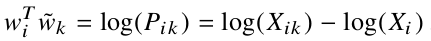
\includegraphics[width=0.6\hsize]{file/eq7.png},通过增加偏置项使得模拟$w_i^T\widetilde{w}_k$与$X_{ij}$之间的关系:\\
    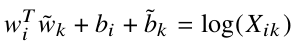
\includegraphics[width=0.5\hsize]{file/eq4.png}
   \end{enumerate}

  \end{columns}

}


\frame{
  \frametitle{GloVe Model}
  \begin{columns}[c]
   \column{0.4\hsize}
   \begin{block}{}
   \begin{itemize}
    \item $X_{ij}:word_j$作为$word_i$上下文出现次数
    \item $X_i=\sum_kX_{ik}$
    \item $P_{ij}=P(j|i)=X_{ij}/X_i$
    \item $F(w_i,w_j,\widetilde{w}_k)=P_{ik}/P_{jk}$
   \end{itemize}
   \end{block}
   
   \column{0.58\hsize}
   \begin{enumerate}
    \item 改用向量差别 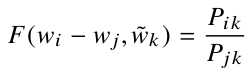
\includegraphics[width=0.4\hsize]{file/eq1.png}
    \item 保持线性结构 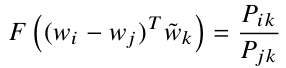
\includegraphics[width=0.45\hsize]{file/eq2.png}
    \item \only<1>{ 我们采用$F=exp$或者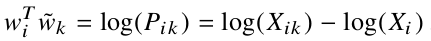
\includegraphics[width=0.5\hsize]{file/eq7.png},使得下面的式子成立\\}
     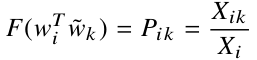
\includegraphics[width=0.35\hsize]{file/eq6.png} 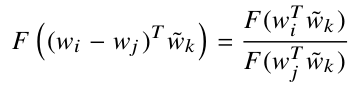
\includegraphics[width=0.5\hsize]{file/eq3.png}
    \item \only<1>{ 如果是采用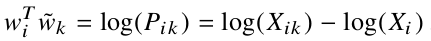
\includegraphics[width=0.6\hsize]{file/eq7.png},通过增加偏置项使得模拟$w_i^T\widetilde{w}_k$与$X_{ij}$之间的关系:\\}
    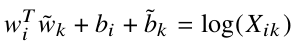
\includegraphics[width=0.5\hsize]{file/eq4.png}
    \only<2,3>{\item 目标函数 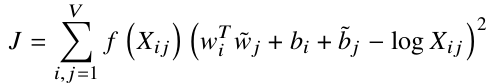
\includegraphics[width=0.6\hsize]{file/eq5.png}}
    \only<3>{
      \\ \vspace{1mm}
      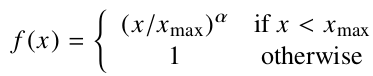
\includegraphics[width=0.6\hsize]{file/fx.png}\\ 
      \vspace{1mm}
      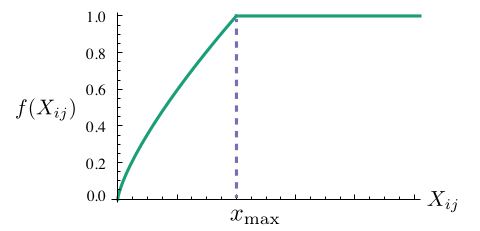
\includegraphics[width=0.6\hsize]{file/fx_fig.png}}
   \end{enumerate}

  \end{columns}

}


\frame{
  \frametitle{GloVe Model}
  GloVe的目标函数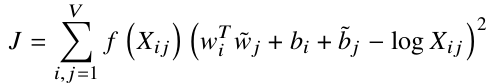
\includegraphics[width=0.4\hsize]{file/eq5.png} 对比window-based methods (skip-gram and ivLBL)的目标函数:
  
  \begin{itemize}
   \only<1>{
   \item 当前词$word_i$预测其上下文单词$word_j$: 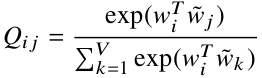
\includegraphics[width=0.3\hsize]{file/eq10.png}
   \item 目标函数为 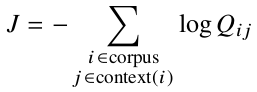
\includegraphics[width=0.3\hsize]{file/eq11.png}
   \item 合并目标函数中的相同项:  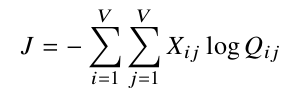
\includegraphics[width=0.3\hsize]{file/eq12.png}
   \item 根据$X_i=\sum_kX_{ik}$, $P_{ij}=P(j|i)=X_{ij}/X_i$,转化目标函数 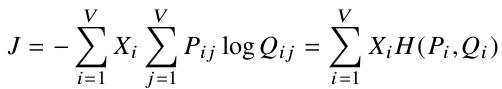
\includegraphics[width=0.4\hsize]{file/eq13.png}
   }
   \only<2>{
   \item 转化目标函数 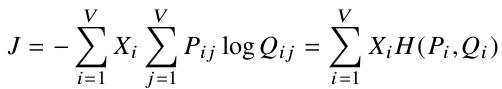
\includegraphics[width=0.3\hsize]{file/eq13.png}
   \item 归一化的$P_{ij}, Q_{ij}$计算复杂,不使用交叉熵,改用压缩过的最小均方误差衡量$P,Q$差别大小
   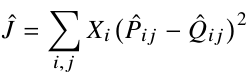
\includegraphics[width=0.2\hsize]{file/eq14.png}  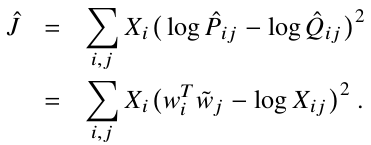
\includegraphics[width=0.3\hsize]{file/eq15.png}
   \item Mikolov提出限制权重来消除高频词的过度影响 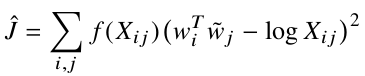
\includegraphics[width=0.3\hsize]{file/eq16.png}
      \begin{itemize}
       \item GloVe的目标函数是合理的(?)
      \end{itemize}

   }
  \end{itemize}

}

\frame{
  \frametitle{GloVe Model}
  复杂度分析
  \begin{itemize}
   \item 
  \end{itemize}

}

\frame{
  \begin{columns}[c]
   \column{.15\hsize}
   \column{.7\hsize}
   \begin{block}{}
    \centering \Large Experiments
   \end{block}

   \column{.15\hsize}
  \end{columns}

}


\frame{\footnotesize
  \frametitle{Experiments}
  Word analogies
  \begin{columns}[c]
   \column{0.5\hsize}
   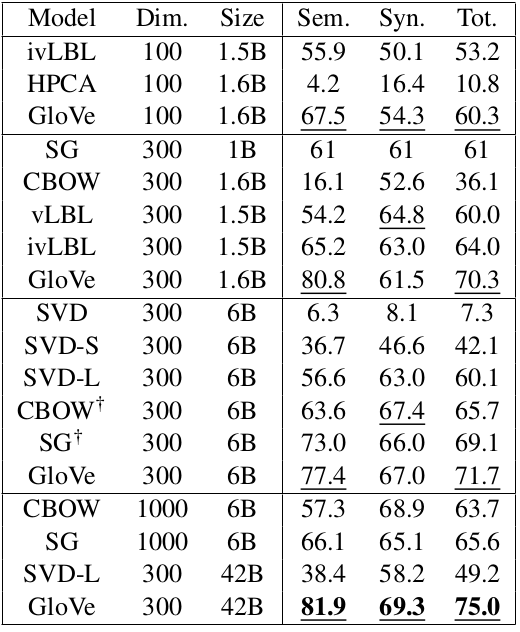
\includegraphics[width=0.9\hsize]{file/word_analogies.png}
   
   \column{0.6\hsize}
  \begin{itemize}
   \item 19544组问题:$a\ is\ to\ b\ as\ c\ is\ to\ \_\_ ?$
   \begin{itemize}
    \item SVD-S:矩阵元素值压缩$\sqrt{X_{trunc}}$
    \item SVD-L:压缩$\log(1+X_{trunc})$
    \item SVD-$f(X)$ ?
   \end{itemize}

   \item CBOW 效果提升不明显
  \end{itemize}
   
  \end{columns}

}


\frame{
  \frametitle{Experiments}
  Word Similarity
  \begin{columns}[c]
   \column{0.65\hsize}
   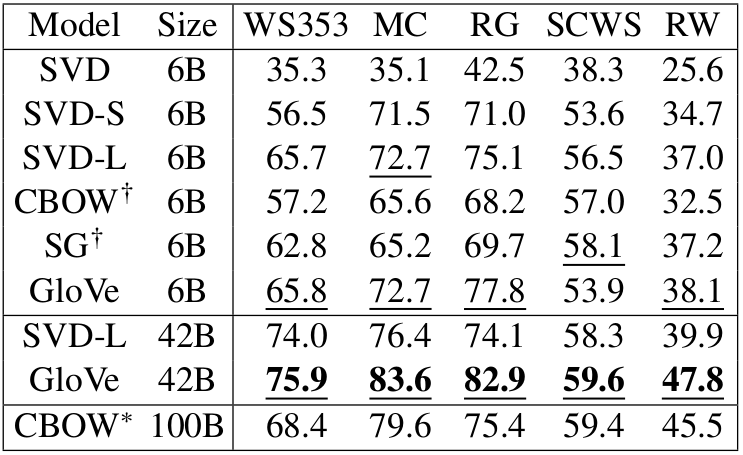
\includegraphics[width=0.9\hsize]{file/word2vec_sim.png}
   
   \column{0.3\hsize}
  \begin{itemize}
   \item 
  \end{itemize}
   
  \end{columns}

}

\frame{
  \frametitle{Experiments}
  NER
  \begin{columns}[c]
   \column{0.55\hsize}
   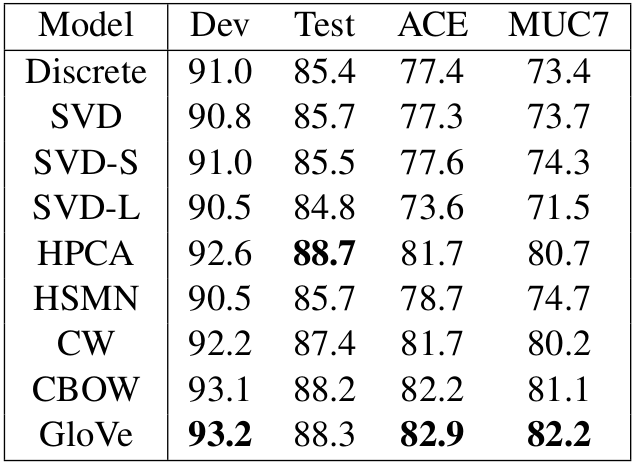
\includegraphics[width=0.9\hsize]{file/word2vec_NER.png}
   
   \column{0.45\hsize}
  \begin{itemize}
   \item Discrete: 直接使用 Stanford NER的输出结果
   \item 20维,窗口大小为5
  \end{itemize}
   
  \end{columns}

}


\end{document}